\section{Aktualny stan wiedzy}

Algorytmy opierające się o sztuczną inteligencję cieszą się dużą popularnością ze względu na ich ogromną gamę zastosowań. Rozwiązania związane z uczeniem maszynowym zrewolucjonizowały w ostatnich dekadach wiele dziedzin nauki i prac badawczych. Technologie te, pozwoliły w niezliczonej liczbie przypadków przewyższyć konkurencyjne rozwiązania pod względem skuteczności i wydajności. 
Świadectwem tego, jest na przykład inteligentne nad-próbkowanie, wydatnie zwiększające jakość obrazów oraz filmów na podstawie jedynie ich kopii o niskiej rozdzielczości. 

Dodatkowo, sztuczna inteligencja umożliwiła opracowanie wielu funkcjonalności, którym klasyczne podejście do programowania nie jest fizycznie w stanie dorównać (w skończonej liczbie instrukcji). Przykładem tego, jest przewidywanie trendów i specyficzne rodzaje detekcji.

\subsection{Istniejące rozwiązania i prace naukowe}

Na dzień dzisiejszy istnieje wiele różnych implementacji systemów wykrywania koloru pojazdów. Reinterpretacji tego problemu pojawia się z biegiem czasu coraz więcej. Fakt ten wynika z rosnącego zainteresowania oraz zapotrzebowania na rozwój algorytmów opartych o uczenie maszynowe w obszarze przetwarzania obrazów, które jest dominującym narzędziem w tej dziedzinie.

Prace naukowe z dziedziny rozpoznawania koloru pojazdów przedstawiają swoiste podejścia do implementacji algorytmu. Proponują oraz uzasadniają przyjętą konfigurację uczenia maszynowego, oferując coraz lepsze wyniki. Twórczość autorów w kwestii optymalizacji algorytmów owocuję nietuzinkową skutecznością i wydajnością otrzymanych rozwiązań.


% Vehicle Color Recognition on Urban Road by Feature Context
% \subsubsection{Regresja liniowa} -> alternatywny podtytuł
\subsubsection{"\null{}Rozpoznawanie koloru samochodów osobowych w ruchu drogowym przez wyodrębnienie cech znaczących" \cite{chen_ref}}
Rozwiązanie opracowane przez Pan Chen, Xiang Bai, Wenyu Liu. Ta praca naukowa jest szczególnie znacząca, ponieważ użyty w niej zbiór danych trenujących jest publicznie dostępny i wiele innych prac naukowych używa go w celach ewaluacyjnych dla swoich rozwiązań.

Kroki zaimplementowany przez kadrę algorytmu to:
\begin{itemize}
    \item Detekcja pojazdu
    \item Usunięcie rozmycia i zamglenia z obrazu
    \item Uwydatnienie kolorów
    \item Wyodrębnienie z obrazu obszaru zainteresowania (ROI, z ang. Region of interest)
    \item Użycie modelu regresji liniowej (SVM, z ang. support vector machine, trenowanej również na ROI pozyskanych z danych uczących) w celu wyznaczenia dominującego koloru w obszarze zainteresowania
\end{itemize}

\begin{figure}[h!]
    \begin{center}
        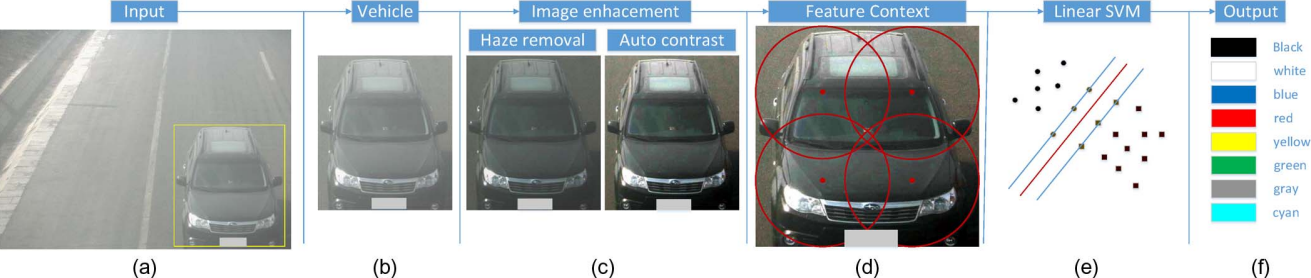
\includegraphics[scale=0.48]{img/chen.png}
    \end{center}
    \caption{Kroki algorytmu: a) obraz wejściowy, b) wynik detekcji i wycięcia, c) kolejno usunięcie zamglenia i uwydatnienie kolorów, d) ROI, e) trenowanie/testowanie modelu SVM, f) wynik działania algorytmu}
    \label{fig:chen_algo}
\end{figure}

Algorytm ten, cieszy się raportowaną przez twórców skutecznością w granicach \textbf{92\%}. Głównym założeniem projektantów, było umożliwienie działania programu zarówno na zdjęciach jak i obrazie wideo. Przetwarzanie wstępne w postaci usuwania niedoskonałości i wyznaczenia ROI jest niezwykle kosztowne pod kątem zasobów sprzętowych. Niska wydajność uniemożliwia satysfakcjonujące działanie algorytmu na obrazie wideo (niska liczba klatek na sekundę). Z tego powodu, został użyty model regresji liniowej. Model ten, jest mniej wymagający sprzętowo w porównaniu do modelu sieci neuronowej. Dzięki temu kompromisowi, autorom udało się uzyskać wysoką skuteczność w połączeniu z zadowalającą wydajnością algorytmu.

% Vehicle Color Recognition using Convolutional Neural Network
% \subsubsection{Splotowa sieć neuronowa}
\subsubsection{"\null{}Rozpoznawanie koloru samochodów osobowych używając splotowej sieci neuronowej" \cite{Su2015/12}}
Podejście zaproponowane przez Reza Fuad Rachmadi oraz Ketut Eddy Purnama.

Algorytm oparty jest na:
\begin{itemize}
    \item Konwersji obrazu do przestrzeni HSV (z ang. Hue Saturation Value) oraz CIELab
    \item Przepuszczenia skonwertowanych obrazów przez splotową sieć neuronową (CNN)
\end{itemize}

\pagebreak

\begin{figure}
    \begin{center}
        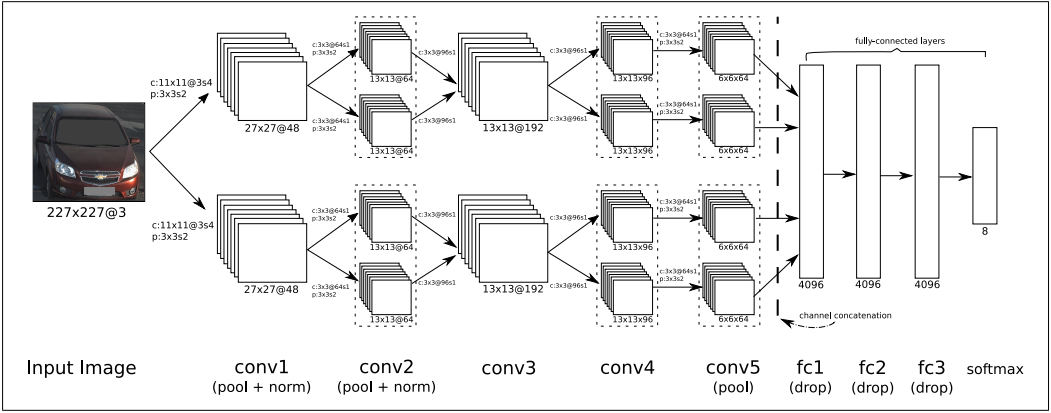
\includegraphics[scale=0.6]{img/cnn_arch.png}
    \end{center}
    \caption{Architektura CNN użytej w pracy naukowej}
    \label{fig:cnn_arch}
\end{figure}

Użyta splotowa sieć neuronowa została wytrenowana według procedury wprowadzonej przez Alexa Krizhevskiego. Polega ona na zmniejszaniu kroku modyfikacji współczynnika uczenia wraz z kolejnymi iteracjami uczenia o stałą wartość (poczynając od pewnej ustalonej iteracji). W przypadku artykułu stała to 10.

Splotowe sieci neuronowe są zazwyczaj używane do klasyfikacji pod kątem kształtu podmiotu. Może ona jednak zostać użyta do klasyfikacji pod względem koloru, dzięki konwersji do przestrzeni uwydatniających rozkład kolorów w obrazie, takich jak HSV oraz CIELab. 

Te zabiegi pozwoliły autorom algorytmu osiągnąć skuteczność 94\%, czyli o 2\% większą od rozwiązania Pan chen, Xiang Bai oraz Wenyu Li, na tym samym zbiorze danych. 

Wadą tego rozwiązania jest czas trenowania modelu CNN, przez co autorzy trenowali i testowali algorytm jedynie na \underline{połowie} obrazów ze zbioru. Nawet mimo tego ograniczenia liczebności danych uczących, trenowanie modelu przebiegało przez okres około 4 dni, używając potężnej karty graficznej w celu zrównoleglenia wymagających operacji.

Z macierzy pomyłek udostępnionej przez twórców rozwiązania, możemy wnioskować z jakimi kolorami algorytm radził sobie najlepiej, a z jakimi miał problemy. Większość kolorów cieszy się wysoką skutecznością rozpoznawania przez model, jednak kolor szary był w około 10\% mylony z kolorem białym, a zielony z szarym oraz czarnym w aż 15\% przypadków testowych.

\begin{figure}[h!]
    \begin{center}
        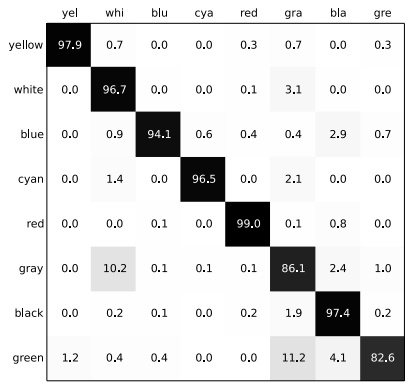
\includegraphics[scale=1.2]{img/confusion_cnn.png}
    \end{center}
    \caption{Macierz pomyłek rozwiązania}    
    \label{fig:confusion_cnn}
\end{figure}

% Vehicle Color Recognition in The Surveillance with Deep Convolutional Neural Networks
% \subsubsection{Głęboka splotowa sieć neuronowa}
% \subsubsection{"\null{}Rozpoznawanie koloru samochodów osobowych w monitoringu ruchu drogowego z użyciem głębokich splotowych sieci neuronowych" \cite{DBLP:journals/corr/RachmadiP15}}

\pagebreak

\subsection{Aplikacje non-profit i open source}
Wiele entuzjastów dziedziny uczenia maszynowego oraz przetwarzania obrazów zdecydowało się na implementację swojej własnej wersji algorytmu wykrywania kolorów pojazdów drogowych. Rozwiązania te, są z reguły dostępne w formie kodu otwartego źródła w publicznych repozytoriach.

Kilka przykładów:
\begin{itemize}
    \item \textbf{Vehicle-Make-Color-Recognition} użytkownika nikalosa. Rozwiązanie napisane w pełni w języku python i bibliotece Pytorch, opiera się na \underline{uczeniu transferowym}. To podejście koncentruje się na zachowaniu wiedzy pozyskanej przez model podczas uczenia i użycie jej w kolejnej operacji uczenia. Użyty model to resnext101 (32x8d). Oprócz koloru, algorytm rozpoznaje również markę pojazdu. \cite{nikalosa}
    
    \item \textbf{car-color-identification} użytkownika sergorl. To implementacja rozpoznawania koloru aut używająca splotowych sieci neuronowych opisanych w \textbf{Keras}, będącej interfejsem do biblioteki Tensorflow. \cite{sergorl}
    
    \pagebreak
    
    \item \textbf{Vehicle-Detection-And-Color-Classification} użytkownika SKsaqlain. Do detekcji samochodów używane jest rozróżnienie statycznych obiektów w kolejnych klatkach obrazu wideo. Po odizolowaniu samochodu z obrazu, używana jest klasyfikacja za pomocą algorytmu centroidów (K-means) na znormalizowanej macierzy kolorów wyodrębnionej z obszaru zajmowanego przez wykryte auto. \cite{saqlain}
\end{itemize}

\subsection{Aplikacje komercyjne}
Istnieje wiele komercyjnych systemów pozwalających na kompleksową identyfikację pojazdów. 
Detekcja koloru samochodu jest używana w tym celu komplementarnie z rozpoznawaniem:
\begin{itemize}
    \item Marki
    \item Modelu
    \item Typu pojazdu (auto osobowe, dostawcze, ciężarowe, dwuślad)
    \item Zawartości tablic rejestracyjnych
\end{itemize}

Kilka przykładowych, komercyjnych systemów pozwalających na kompleksową identyfikację pojazdów to: 
\begin{itemize}
    \item \textbf{Carmen® MMR} firmy \textbf{Adaptive Recognition} (wcześniej znanej jako ARH) \cite{carmen}
    \item \textbf{Asura} firmy \textbf{Milestone Systems A/S} \cite{asura}
    \item \textbf{numberOK SDK LPR} firmy \textbf{FF Group} \cite{numberok}
    \item Rozwiązanie firmy \textbf{Kuartis} (implementuje jedynie rozpoznawanie koloru i tablic rejestracyjnych pojazdów) \cite{kuartis}
\end{itemize}
